\DiaryEntry{Prefix Codes - Intuition}{2021-04-26}{Coding}

We consider prefix codes and play around with some examples. We start with a code for $3$ symbols as in the folloing Figure, upper part.

This is a prefix code as all codewords are at the leaves of the tree. We continue using the convention from the previous entry that a left turn corresponds to a $0$ and a right turn corresponds to a $1$. So the codeword for symbol $B$ is $01$ (left-right).

\begin{figure}[H]
    \centering
    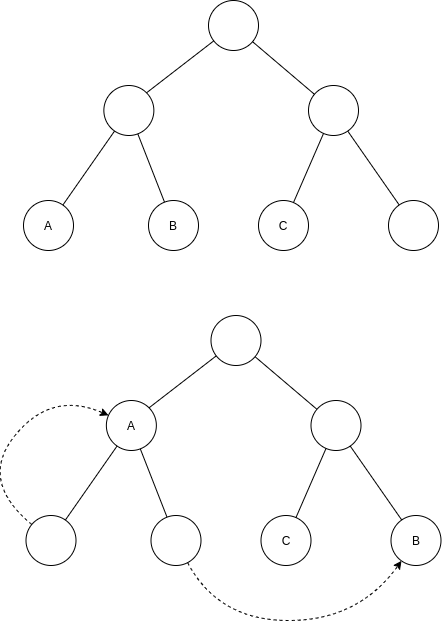
\includegraphics[scale=0.4]{images/2021-04-26-scenario_1.png}
\end{figure}

Assume that symbol $A$ has a higher probability and we decide to assign it a shorter codeword. We therefore move it up in the tree (see lower part of the Figure) so that the codeword becomes $0$. Since we want a prefix code, we have to move symbol $B$ from its current position so that it does not stay below $A$. We therefore move $B$ to a currently unused tree node (codeword $11$).

As a whole, the average codeword length has decreased: Symbols $B, C$ have codewords of the same length assigned and symbol $A$ has a codeword of length $1$ assigned.

This example was easy, as we had enough room in the tree to accomodate symbol $B$. The next example is a bit more involved.

The initial assignment is shown in the upper part of the following Figure. We again decide to assign symbol $A$ the shorter codeword $0$ (instead of $000$). Now we have to move symbols $B, C, D$ to another place in the tree. We move symbol $B$ from $001$ to $110$. Symbols $C$ and $D$ are a bit more complex as we have only one more vacancy with codelength $3$ in the tree. We therefore need to introduce a further level in the tree and move symbol $C$ to $1110$ and symbol $D$ to $1111$.

\begin{figure}[H]
    \centering
    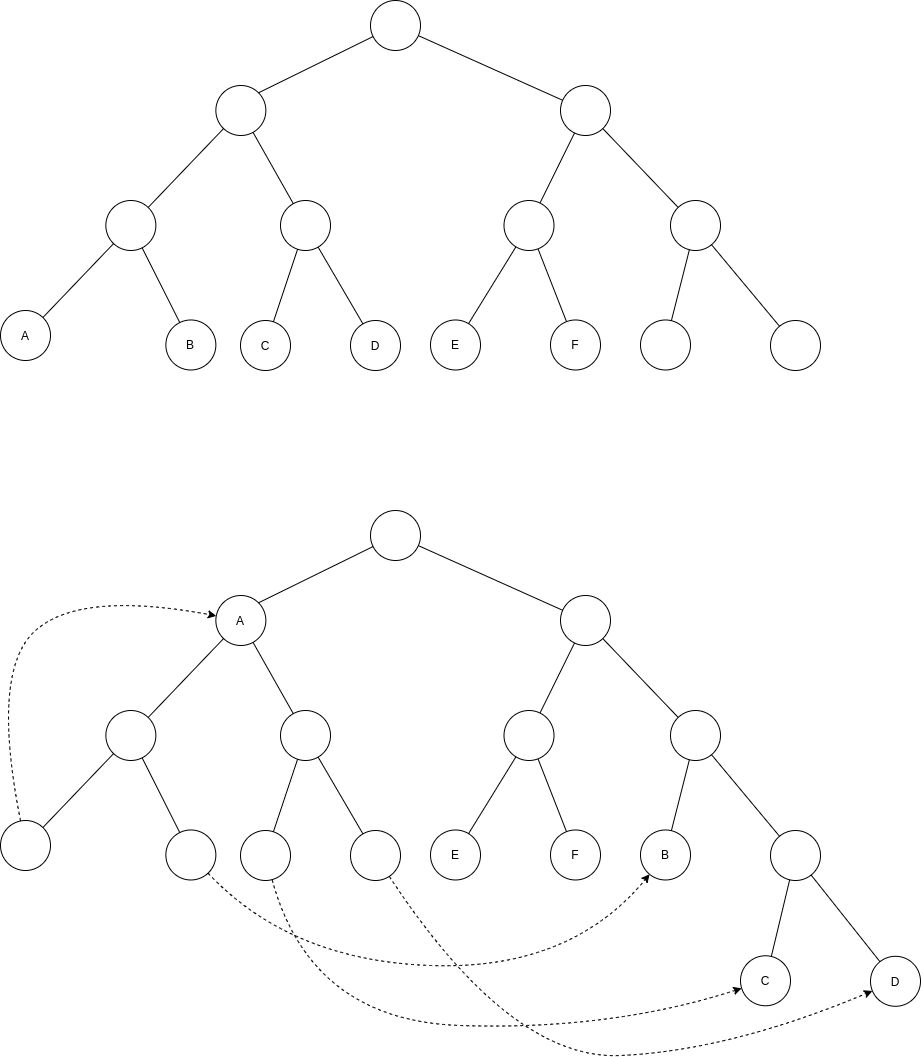
\includegraphics[scale=0.4]{images/2021-04-26-scenario_2.png}
\end{figure}

In this case, we cannot make a statement about the average codeword length: We have shortened the codeword for symbol $A$, however, the codeword length for symbols $C, D$ has increased. Without knowing the symbol probabilities, we cannot say which effect is stronger.

In addition, maybe it would have been better to move another symbol to where we have moved symbols $C$ and $D$ and / or restructure the tree more fundamentally. The Huffman code construction starts bottom-up (i.e. with the symbols having lowest probability first) and does not rework an already existing tree. Therefore a Huffman code may yield a different result in this case.



%%% Local Variables:
%%% mode: latex
%%% TeX-master: "journal"
%%% End:
